\documentclass{article}
\usepackage{graphicx} % Required for inserting images
\usepackage{float}
\usepackage[T1]{fontenc}
\usepackage{amsmath}
\usepackage[margin=1in]{geometry}
\usepackage{booktabs}
\usepackage{tabularx}
\usepackage[hidelinks]{hyperref}

\title{A trend-gated hedge band for long calls on the gamma book}
\author{Experiment report \textperiodcentered{} L/S Gamma Desk, QUANTT}
\date{2026-11-11}

\begin{document}

\maketitle

\textbf{Question:} When the book holds a long call and SPY is trending, does letting the share hedge drift up to 30 shares before re-hedging give higher net P\&L than re-hedging every share? The test is at 1x and 2x spreads, over the full window and in each half, without a worse tail.

\textbf{Method:}

\begin{itemize}

\item \textbf{Pre-registered backtest:} the research switch was committed first (a837054), then the hypothesis card, config and script (a8ac9e0), before any registered run.

\item \textbf{Data:} the live paper rules (\texttt{configs/\allowbreak{}paper.\allowbreak{}toml}) are replayed on R2 replay snapshots v1 (config\_hash b040760187f0) over the development window 2014-06-02 to 2024-12-31. The out-of-sample window (2025-01-01 to 2026-07-10) was not used.

\item \textbf{Regime detector:} the 10-day Kaufman efficiency ratio of SPY's daily closes, using completed days only: the size of the 10-day move divided by the sum of the daily moves. It is 1 for a straight line and near 0 for chop. ``Trending'' means a ratio of at least 0.4, in either direction.

\item \textbf{Rule:} at each daily hedge time, if the book holds a long call and the detector says trending, the engine skips any rebalance smaller than the wider band and logs it as a held hedge. Otherwise it re-hedges every share, as the paper rules do. Short puts are never affected.

\item \textbf{Variants:}

\begin{itemize}

\item \texttt{trend30}: 30-share band in a trend (\texttt{long\_\allowbreak{}hedge\_\allowbreak{}band = 30}, \texttt{trend\_\allowbreak{}er = 0.\allowbreak{}4}). \textbf{Primary.}

\item \texttt{always30}: the same 30-share band on every long-call day, with no detector (\texttt{trend\_\allowbreak{}er = 0}). A control.

\item \texttt{trend15}: a 15-share band in a trend. A sensitivity.

\end{itemize}

\item \textbf{Comparison:} the baseline (current paper rules, re-hedging every share), at the same spread multiple. A fresh baseline trial was run because the registered one no longer matched the config. The only changes were two live-only order settings (option slippage and the share-order pad), which the backtest does not read; the fresh run reproduces the old one exactly.

\item \textbf{Runs:} every variant was run at 1x and 2x spreads. Costs: \$0.65 per contract and \$0.005 per share, with a \$1 minimum per order. Exits and hedges run once a day at 10:15 ET.

\end{itemize}

This report was written by Claude at the PM's request.

\section{Result vs the pass bar}

Every check had to hold at both 1x and 2x. P\&L is in USD for one contract; ES 5\% is the mean of the worst 5\% of daily net P\&L.

\begin{center}\small
\begin{tabularx}{\linewidth}{>{\raggedright\arraybackslash}X l >{\raggedright\arraybackslash}X l >{\raggedright\arraybackslash}X l}
\toprule
\textbf{Check} & \textbf{1x value} & \textbf{1x bar} & \textbf{2x value} & \textbf{2x bar} & \textbf{Result} \\
\midrule
Net P\&L, full window & \ensuremath{-}\$2,177 & > \ensuremath{-}\$2,060 & \ensuremath{-}\$4,239 & > \ensuremath{-}\$4,122 & fail \\
Net P\&L, 2014-06 to 2019-12 & \ensuremath{-}\$989 & > \ensuremath{-}\$986 & \ensuremath{-}\$1,514 & > \ensuremath{-}\$1,511 & fail \\
Net P\&L, 2020-01 to 2024-12 & \ensuremath{-}\$1,188 & > \ensuremath{-}\$1,073 & \ensuremath{-}\$2,725 & > \ensuremath{-}\$2,611 & fail \\
ES 5\% (daily), full window & \ensuremath{-}\$100.6 & \ensuremath{\leq} \$106.1 in size & \ensuremath{-}\$108.5 & \ensuremath{\leq} \$115.0 in size & pass \\
\bottomrule
\end{tabularx}
\end{center}

The event floor was met: \texttt{trend30} held back 37 hedges at 1x (floor 30).

\textbf{Verdict: failed.} The trend-gated band made \$118 less than re-hedging every share over ten and a half years at 1x (\$117 at 2x), and it was behind in both halves. The book still loses money either way.

\subsection{Full-window numbers (not part of the bar)}

\begin{center}\small
\begin{tabularx}{\linewidth}{>{\raggedright\arraybackslash}X l l l l l l}
\toprule
\textbf{} & \textbf{baseline 1x} & \textbf{trend30 1x} & \textbf{always30 1x} & \textbf{trend15 1x} & \textbf{baseline 2x} & \textbf{trend30 2x} \\
\midrule
Net P\&L & \ensuremath{-}\$2,060 & \ensuremath{-}\$2,177 & \ensuremath{-}\$1,881 & \ensuremath{-}\$1,704 & \ensuremath{-}\$4,122 & \ensuremath{-}\$4,239 \\
Sharpe & \ensuremath{-}0.36 & \ensuremath{-}0.36 & \ensuremath{-}0.30 & \ensuremath{-}0.29 & \ensuremath{-}0.68 & \ensuremath{-}0.68 \\
Max drawdown & \$3,027 & \$3,129 & \$3,058 & \$2,945 & \$4,258 & \$4,375 \\
ES 5\% (daily) & \ensuremath{-}\$96.5 & \ensuremath{-}\$100.6 & \ensuremath{-}\$105.7 & \ensuremath{-}\$97.3 & \ensuremath{-}\$104.5 & \ensuremath{-}\$108.5 \\
Round trips & 131 & 131 & 131 & 131 & 131 & 131 \\
Commissions (options /\allowbreak{} hedges) & \$262 /\allowbreak{} \$914 & \$262 /\allowbreak{} \$875 & \$262 /\allowbreak{} \$789 & \$262 /\allowbreak{} \$879 & \$262 /\allowbreak{} \$914 & \$262 /\allowbreak{} \$875 \\
Hedges held back & 0 & 37 & 127 & 33 & 0 & 37 \\
\bottomrule
\end{tabularx}
\end{center}

\section{Charts}

\begin{figure}[H]\centering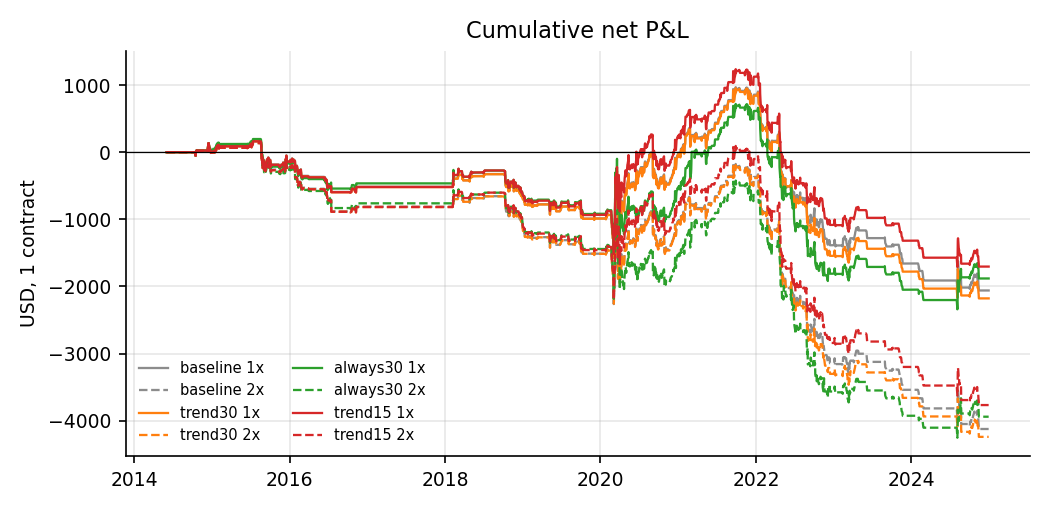
\includegraphics[width=0.92\linewidth]{figures/cum_pnl.png}\caption{Cumulative net P\&L, 1x solid and 2x dashed; baseline grey}\end{figure}

The four books are almost the same line. They separate only from March to mid-2020 and in 2021-2024, where the wider bands held back the most hedges. \texttt{trend30} ends just below the baseline at both spreads.

\begin{figure}[H]\centering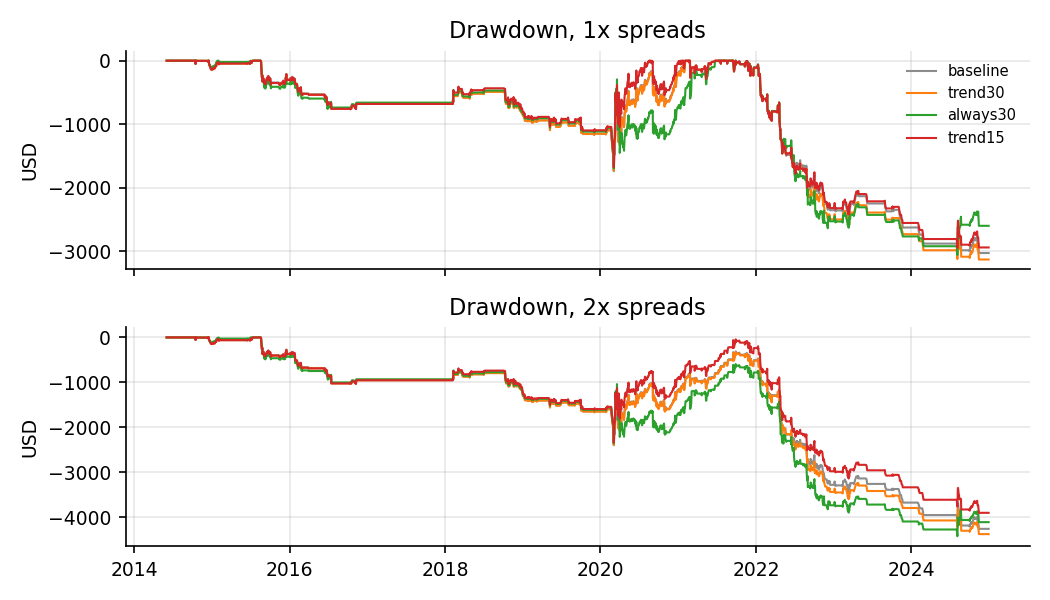
\includegraphics[width=0.92\linewidth]{figures/drawdown.png}\caption{Drawdown at 1x and 2x spreads}\end{figure}

Drawdowns match until 2020. \texttt{always30} stays deepest under water from April 2020 into 2021, and \texttt{trend30} ends with a slightly larger maximum drawdown than the baseline (\$3,129 against \$3,027 at 1x).

\begin{figure}[H]\centering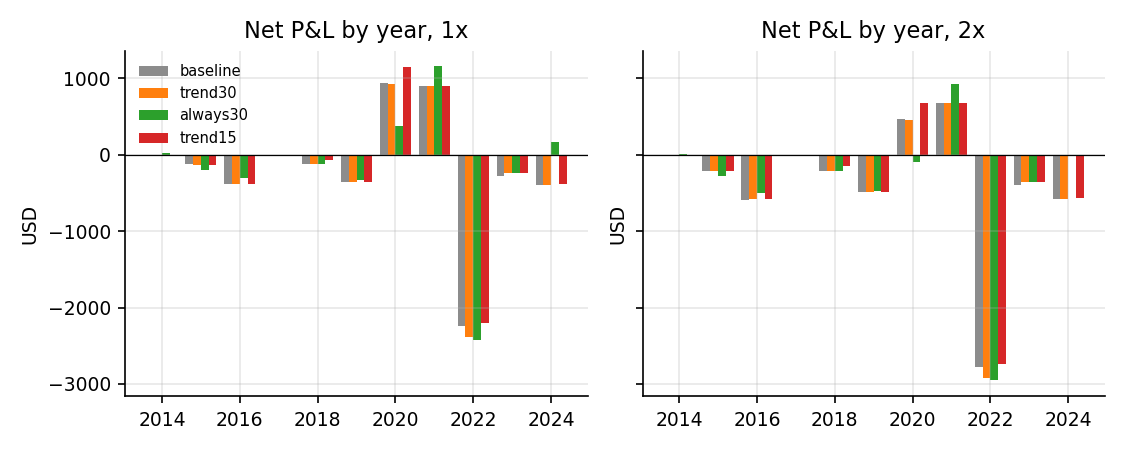
\includegraphics[width=0.92\linewidth]{figures/yearly.png}\caption{Net P\&L by year}\end{figure}

2022 is every book's worst year (about \ensuremath{-}\$2.2k to \ensuremath{-}\$2.4k at 1x), and \texttt{trend30} loses \$142 more than the baseline there. Across the other years, \texttt{trend30} is within \$40 of the baseline. \texttt{always30} swings more: \ensuremath{-}\$565 against the baseline in 2020, then +\$254 in 2021 and +\$569 in 2024.

\begin{figure}[H]\centering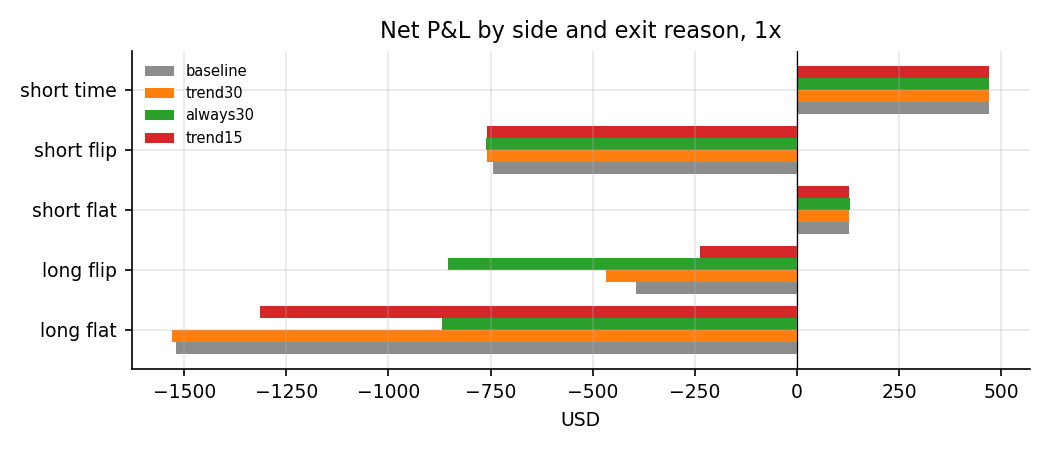
\includegraphics[width=0.92\linewidth]{figures/by_reason.png}\caption{Net P\&L by side and exit reason, 1x}\end{figure}

The short-put bars are almost identical across books, because the rule never touches puts. All the differences sit in the long-call rows, where the books trade the same calls but hedge them differently.

\begin{figure}[H]\centering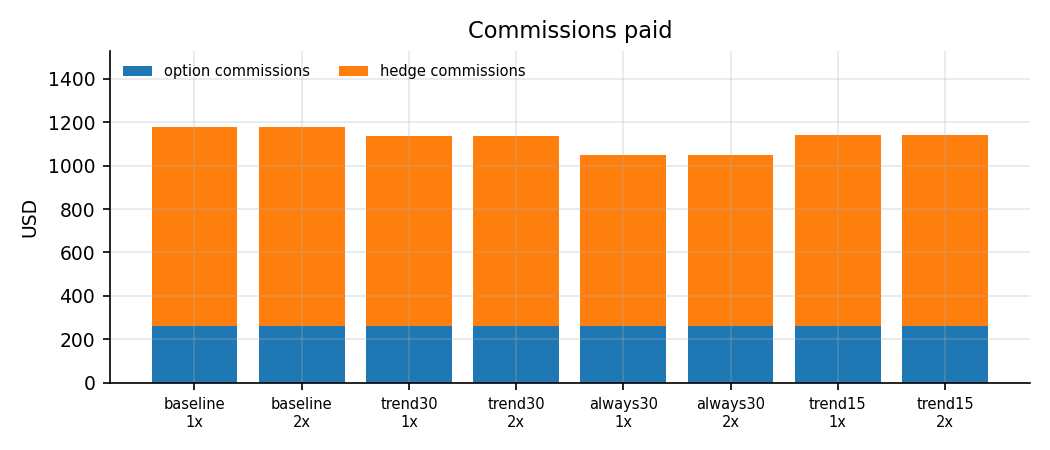
\includegraphics[width=0.92\linewidth]{figures/fees.png}\caption{Commissions paid}\end{figure}

Hedge commissions fall with every held hedge: \$39 saved for \texttt{trend30}, \$125 for \texttt{always30} and \$35 for \texttt{trend15}. Option commissions are unchanged (\$262) because the trades are identical.

\begin{figure}[H]\centering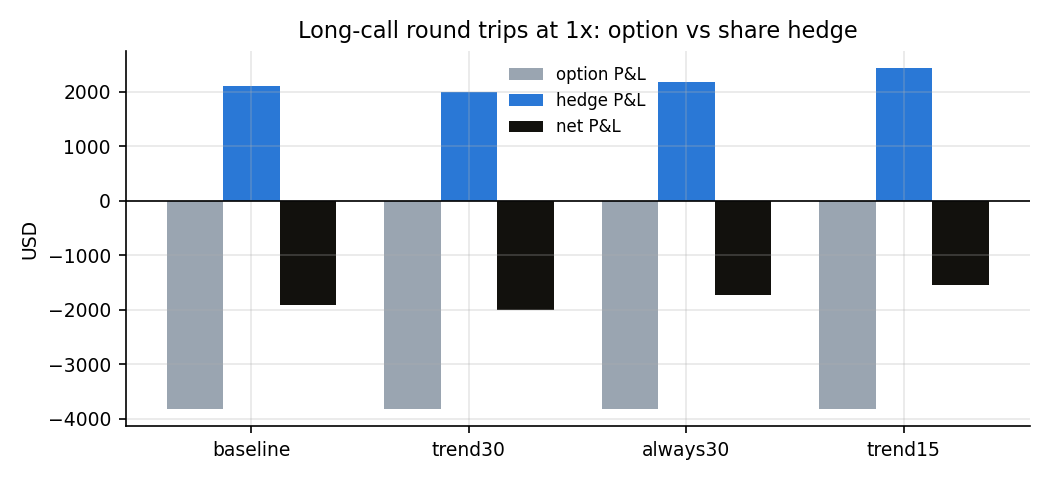
\includegraphics[width=0.92\linewidth]{figures/long_split.png}\caption{Long-call round trips at 1x: option vs share hedge}\end{figure}

This is the main chart. On the 30 long-call round trips, the calls lost \$3,822 in every book, and the share hedge made money in every book: +\$2,115 in the baseline and +\$1,996 with \texttt{trend30}. Hedging was not what lost money on the long side; the calls were.

\begin{figure}[H]\centering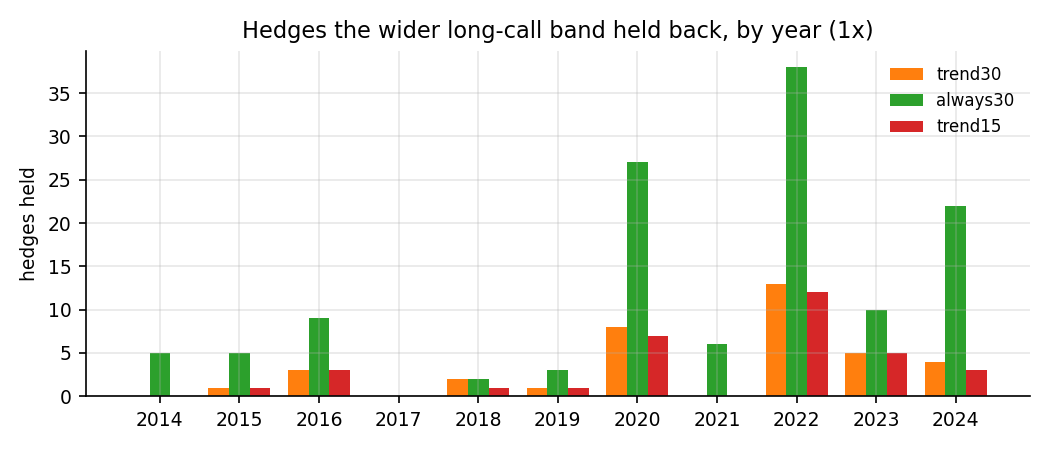
\includegraphics[width=0.92\linewidth]{figures/trend_holds.png}\caption{Hedges the wider long-call band held back, by year (1x)}\end{figure}

The detector-gated bands held back 33-37 hedges over the whole window, most of them in 2020 and 2022. The always-on band held back 127.

\section{Analysis}

\textbf{The trades are identical; only the hedges differ.} All four books open and close the same 131 positions on the same days, strikes and exit reasons, at both spreads. The long-call stop uses option plus hedge P\&L, so the band could in principle have moved a stop, but no book had a stop exit: every exit is a flat, flip or time exit. Every P\&L difference therefore comes from the share hedge and its commissions. For \texttt{trend30} at 1x, the \ensuremath{-}\$118 splits into:

\begin{itemize}

\item \ensuremath{-}\$82 on the long-call round trips;

\item \ensuremath{-}\$13 on short puts, from shares carried over after a long call closed;

\item the rest, about \ensuremath{-}\$24, on share trades outside any round trip.

\end{itemize}

\textbf{The long side loses on the calls, not on the hedge.} Over the 30 long-call round trips, the share hedge made +\$2,115 in the baseline, against \ensuremath{-}\$3,822 on the calls. That's what delta hedging a long-gamma position should do: sell into rallies and buy dips, recovering part of the time decay. Hedging less can only help if the moves you stop hedging keep going. On the paper account in November, a long call hedged with short SPY lost on the shares during a rally. Over 2014-2024, that is the exception: on average the hedge earned money.

\textbf{The detector didn't find trends that continue.} Here each day's P\&L difference is assigned to the regime on the day the hedge was set. Over the 47 holding intervals that started on a trending day while a long call was held, \texttt{trend30} lost \$262 against the baseline. Over the same intervals, \texttt{trend15} gained \$250 and \texttt{always30} lost \$70. The same detector gives opposite signs at 15 and 30 shares, which points to a few individual paths, not a trend effect. A 10-day efficiency ratio above 0.4 does not, on this sample, predict that SPY keeps moving the same way the next day.

\textbf{The differences are small and look like noise.} \texttt{trend30} changed the result of 15 long-call round trips, by \ensuremath{-}\$5 each on average (t = \ensuremath{-}0.23). The two largest changes (+\$238 and \ensuremath{-}\$235) are each bigger in size than the \ensuremath{-}\$82 net. The two variants that beat the baseline are no more convincing:

\begin{itemize}

\item \texttt{always30}: +\$179, t = 0.21 over 30 changed trips;

\item \texttt{trend15}: +\$356, t = 1.34 over 15 changed trips.

\end{itemize}

Neither result is reliable. Most of \texttt{always30}'s gain is saved commissions (\$125 of \$179). Two trades make up most of \texttt{trend15}'s: +\$238 and +\$96 are \$334 of its \$360 on long calls.

\section{Verdict}

\textbf{Failed}, per the pre-registered bar: \texttt{trend30} made less than the baseline over the full window and in both halves, at 1x and 2x, though its tail was within the guard.

Next step: archive this card. A regime-gated hedge for long calls could be retried with a detector that predicts next-day continuation, not just past trend. That would need its own card, and the long side's small sample (30 round trips) would make any edge hard to see. The bigger lever on the long side is the calls themselves, which lost \$3.8k; the 2026-10-16 short-only card already tested dropping them.

\section{Caveats}

\begin{itemize}

\item \textbf{In-sample:} the idea came from the live paper book and the 2026-10-16 short-only result on this window. The detector's 0.4 threshold and 10-day lookback were picked from the feature distribution on this window (about a third of days flagged), not from P\&L. A failure here needs no out-of-sample run.

\item \textbf{One contract:} the \$1 minimum per order is large relative to size. Saved hedge orders are worth \$1 each: that's most of \texttt{always30}'s gain (\$125 of \$179), but not \texttt{trend15}'s (\$35 of \$356).

\item \textbf{Spread model:} fitted on about two weeks of calm 2026 live quotes; the 2x run is the stress test.

\item \textbf{Data gaps:} R2 has no month-end weekdays, so about 3.3\% of scheduled times are skipped.

\item \textbf{Few events:} 30 long-call round trips over 190 trading days (entry to exit), and 37 held hedges for the primary. The floor was met, but any effect of this size is within noise.

\item \textbf{Spot and timing:} spot comes from put-call parity on a 30-minute grid (10:15-15:45), hedges run once a day at 10:15, and the detector sees closes up to the previous day.

\end{itemize}

\section{Trials}

6 trials for this experiment (3 variants \ensuremath{\times} 1x and 2x, one run of \texttt{experiment.\allowbreak{}py}), plus 2 for the fresh baseline, which brings the baseline to 4. The registry now has 148 rows, none on the out-of-sample window. All 8 new rows are tagged with the pre-registration commit a8ac9e0. The pass bar was not changed.

\end{document}
